\documentclass[a4paper,12pt]{scrartcl}

\usepackage{bm,amsmath,url,graphicx}
\usepackage{palatino}
\usepackage{color, xcolor}
\usepackage{listings}


\newcommand{\n}{{\bf n}}
\newcommand{\h}{{\bf h}}
\newcommand{\x}{{\bf x}}
\newcommand{\HH}{{\bf H}}
\newcommand{\thb}{{\boldsymbol{\theta}}}
\newcommand{\python}{{\fbox{\texttt{\bfseries python}}\quad}}
\newcommand{\pen}{{\fbox{\texttt{\bfseries pen\&paper}}\quad}}

\renewcommand{\familydefault}{\rmdefault}


\begin{document}
\section*{\bf SGN-41007 Pattern Recognition and Machine Learning}
\emph{Exercise Set 3: January 25.1--27.1.2017}
\bigskip
\sloppy

\lstdefinestyle{mystyle}{
  belowcaptionskip=1\baselineskip,
  breaklines=true,
  frame=single,
  xleftmargin=\parindent,
  language=Python,
  showstringspaces=false,
  basicstyle=\ttfamily,
  keywordstyle=\bfseries\color{green!40!black},
  commentstyle=\itshape\color{purple!40!black},
  identifierstyle=\color{blue},
  stringstyle=\color{orange},
  moredelim=**[is][\color{red}]{@}{@},
}

\lstset{language=Python,style=mystyle} 


\noindent
Exercises consist of both pen\&paper and computer assignments.
Pen\&paper questions are solved at home before exercises, while
computer assignments are solved during exercise hours. The
computer assignments are marked by text \python and 
Pen\&paper questions by text \pen

\begin{enumerate}

\item \pen \emph{Design an optimal detector for step signal.}

The lecture slides describe an optimal detector for a known waveform $s[n]$.
Apply it to design the optimal detector for a step edge:
\[
s[n] = \begin{cases}
-1, & \text{ for } 0\le n < 10\\
1, & \text{ for } 10\le n < 20
\end{cases}
\]
Simplify the expression as far as you can.

\item \python \emph{Implement a sinusoid detector.}

In this exercise we generate a noisy sinusoid with known frequency and see how
the sinusoid detector of the lecture slides performs.

\begin{enumerate}
	\item Create a vector of zero and sinusoidal components that looks like the plot below.
	Commands: \verb+np.zeros+, \verb+np.concatenate+. Sinusoid is generated by
	\verb+np.cos(2 * np.pi * 0.1 * n)+.
	
	{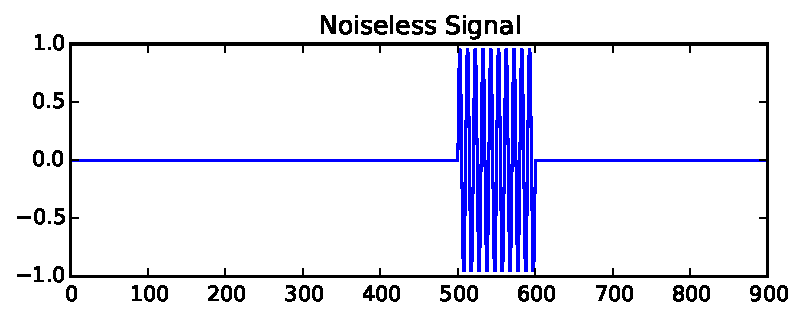
\includegraphics[width=0.7\textwidth]{sinusoid.pdf}}
	
	\item Create a noisy version of the signal by adding Gaussian noise with variance 0.5:
	\verb|y_n = y + np.sqrt(0.5) * np.random.randn(y.size)|.
	
	\item Implement the two detectors and reproduce the below plot.
	
		{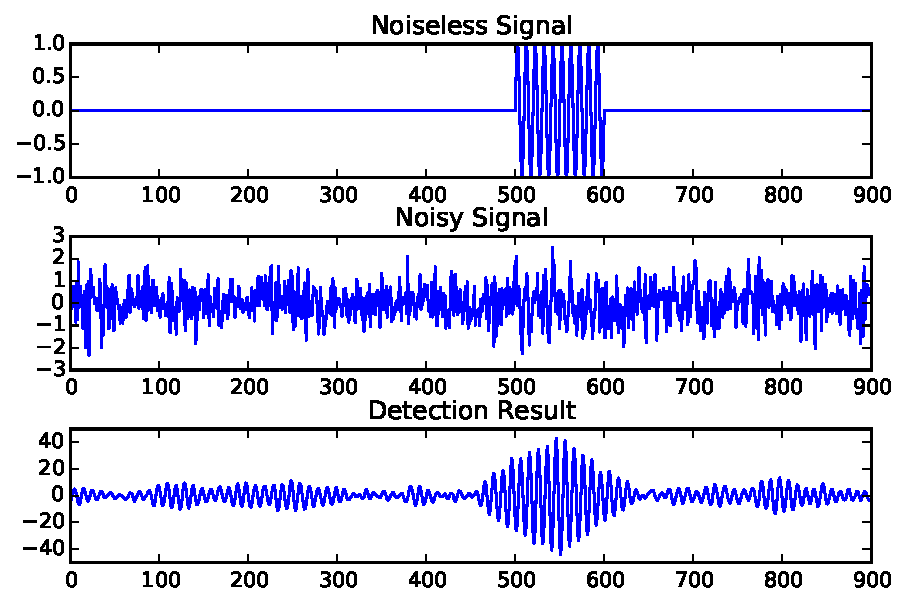
\includegraphics[width=0.7\textwidth]{sinusoidDetection.pdf}}
		
\end{enumerate}



\item \python \emph{Same as previous but different frequency and detector.}

Change the code of the previous exercise such that the frequency is 0.03 and
the detector is the random signal version.

	\qquad	{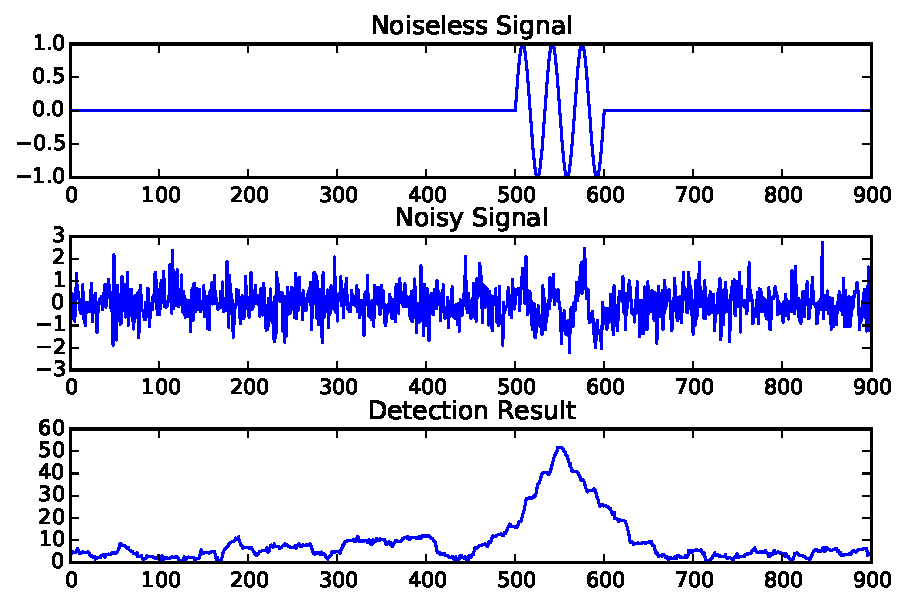
\includegraphics[width=0.7\textwidth]{rayleighSinusoid.pdf}}
		
\item \python \emph{Load a dataset of images split to training and testing.}
\label{ex1}

We will train a classifier to classify hand written digits.
Scikit-learn provides a number of sample datasets.
Load the \verb+digits+-dataset as follows.

\begin{lstlisting}
 from sklearn.datasets import load_digits
 digits = load_digits()
\end{lstlisting}

The result is a \verb+dict+ structure that can be accessed using
\emph{keys}. Find all keywords of the dict with \verb+print(digits.keys())+.
The interesting ones for us are: \texttt{'images'}, \texttt{'data'} and \texttt{'target'}.

Plot the first image of the 1797 numbers like this.
\begin{lstlisting}
 import matplotlib.pyplot as plt 
 plt.gray() 
 plt.imshow(digits.images[0])
 plt.show() 
\end{lstlisting}
Check that this corresponds to the label \verb+digits.target[0]+.

The images are vectorized as rows in the matrix \verb+digits.data+,
whose size is $1797\times 64$ (1797 images of size $8\times 8$).

Split the data to training and testing sets, such that the training
set consists of 80\% and test set 20\% of the data. Use
\verb+sklearn.cross_validation.train_test_split+ to do this and
create variables \verb+x_train+, \verb+y_train+, \verb+x_test+, \verb+y_test+.

\item \python \emph{Train a classifier using the image data.}

In this exercise we will train a nearest neighbor classifier with the data arrays of exercise \ref{ex1}.

\begin{itemize}
\item Initiate a KNN classifier with 
\begin{lstlisting}
from sklearn.neighbors import KNeighborsClassifier
clf = KNeighborsClassifier()
\end{lstlisting}
\item Train the classifier using the training data.
\item Predict the labels for the test data.
\item Compute the accuracy using \verb+sklearn.metrics.accuracy_score+.
\end{itemize}

\end{enumerate}

\end{document}          
